\input{./econtexRoot}\input{\econtexRoot/LaTeX/econtexPaths} 
\documentclass[titlepage]{\econtex} 
\usepackage{xr-hyper}
\usepackage{graphicx}
\usepackage{float}
\graphicspath{ {./Pictures/} }
\input{\econtexRoot/LaTeX/econtexPaths}

\input{\ResourcesDir/owner}

\providecommand{\texname}{CulturalChangeAsLearning}
\usepackage{\LaTeXFiles/BufferStockTheory}

\begin{document}

\providecommand{\versn}{}
\ifthenelse{\boolean{ifWeb}}{  \renewcommand{\ushort}{\underline}\renewcommand{\versn}{Web} }{} 

\hfill{\tiny \jobname~\versn~\today~{at} \DTMcurrenttime, \input{\ResourcesDir/.git-source-commit}~~\input{\ResourcesDir/.git-public-commit}}

\title{Cultural Change as Learning: The Evolution of Female Labor Force Participation over a Century}

\author{Raquel Fernandez \\ Ballpark by: Wonsik Ko\authNum}

\keywords{female labor force participation; cultural transmission; preference formation; learning; S shape; social norms; beliefs}

\jelclass{J16, J21, Z1, D19\\
  \href{https://econ-ark.org}{\includegraphics{\ResourcesDir/PoweredByEconARK}}
}

\renewcommand{\forcedate}{October 16, 2020}
\date{\forcedate}

\maketitle 
\hypertarget{abstract}{}
\begin{abstract}
 This paper investigates the role of changes in culture in generating the dramatic increase in married women's labor force participation over the last century. It develops a dynamic model of culture in which individuals hold heterogeneous beliefs regarding the relative long-run payoffs for women who work in the market versus the home. These beliefs evolve endogenously via an intergenerational learning process. Women are assumed to learn about the long-term payoffs of working by observing (noisy) private and public signals. This process generically generates the S-shaped figure for female labor force participation found in the data. I calibrate the model to several key statistics and show that it does a good job in replicating the quantitative evolution of female LFP in the US over the last 120 years. I also examine the model's cross-sectional and intergenerational implications. The model highlights a new dynamic role for changes in wages via their effect on intergenerational learning. The calibration shows that this role was quantitatively important in several decades.
\end{abstract}

\begin{authorsinfo}
  \name{Contact: \href{mailto:}{\texttt{wko5@jhu.edu}}, Department of Economics, Wyman Hall, Johns Hopkins University, Baltimore, MD 21218, \url{https://github.com/wko5/ballpark/models/We-Would-Like-In-Econ-ARK}}
\end{authorsinfo}

\newcommand{\thankstext}{Thank you to Prof. Christopher D. Carroll for the template on which this paper is written.}

\ifthenelse{\boolean{ifWeb}}{}{\thanks{\thankstext}}

\titlepagefinish

\ifthenelse{\boolean{ifWeb}}{\medskip \noindent {\tiny
    \thankstext \medskip \medskip \medskip
  }}{\pagebreak 
}

\ifthenelse{\boolean{ifWeb}}{\medskip \noindent {\footnotesize \thankstext} \\  {\centering \medskip \medskip \medskip  \noindent \hrule height 0.4pt depth 0.0pt width \textwidth \relax}}{\pagebreak } % \end{Web}

\hrule height 0.4pt depth 0.0pt width \textwidth \relax

\medskip \medskip

\hypertarget{Summary}{}
\section{Summary}

This paper investigates the role of changes in culture in generating the dramatic increase in married women's labor force participation over the last century. 

It develops a dynamic model of culture in which individuals hold heterogeneous beliefs regarding the relative long-run payoffs for women who work in the market versus the home.

These beliefs evolve endogenously via an intergenerational learning process.

It calibrates the model to several key statistics and show that it does a good job in replicating the quantitative evolution of female
LFP in the US over the last 120 years.

The model highlights a new dynamic role for changes in wages via their effect on intergenerational learning.

\hypertarget{The Model}{}
\section{The Model}

\hypertarget{The Work Decision}{}
\subsection{The Work Decision}

\begin{align*}
U(w_{f}, w_{h}, v_{i})&=\frac{c^{1-\gamma}}{1-\gamma}-\textbf{1} (E_{i t}v_i)\\
c = w_h + \textbf{1} w_f,   v_i &=l_i + B_i , B_i = \beta + u_i , E(u_i)=0
\end{align*}

* $\textbf{1}$: an indicator function that takes the value one if she works.

* $w_f$: a woman's earning

* $w_h$: a husband's earning

* $l_i$: a known idiosyncratic component of disutility of working with distribution in the population G(l)

* $B_i$: an individual-level realization of a random variable that is iid across women

* Consumption is a household public good

* $\beta \in \{\beta_H, \beta_L\}$, $\beta_H >\beta_L \geq 0$

Prior to making her work decision, a woman inherits her mother's private signal $s_i$ that yields information about true $\beta$.

\begin{align*}
s_i = \beta + \epsilon_i
\end{align*}
where $\epsilon \sim N(0,\sigma_{\epsilon}^2)$

After inheriting her private signal $s_i$, each woman updates her prior belief using Bayes' rule.

Consider a woman i in period t who has a prior belief about $\beta$ as summarized in the log likelihood ratio (LLR) $\lambda_t = ln \frac{P(\beta=\beta_L)}{P(\beta=\beta_H)}$. By Bayes rule, her beliefs given her private signal s can be summarized in a new LLR, $\lambda_{i t}(s)$ given by

\begin{align*}
\lambda_{i t}(s)=\lambda_t + ln(\frac{P(s|\beta=\beta_L)}{P(s|\beta=\beta_H)})=\lambda_t - (\frac{\beta_H - \beta_L}{\sigma_{\epsilon}^2})(s-\bar{\beta})
\end{align*}
where $\bar{\beta}=(\beta_H+\beta_L)/2$, $s \sim N(\beta, \sigma_{\epsilon}^2)$, $\lambda_{it} \sim N(\lambda_t - (\frac{\beta_H-\beta_L}{\sigma_{\epsilon}^2})(\beta - \bar{\beta}), \frac{(\beta_H-\beta_L)^2}{\sigma_{\epsilon}^2})$

Woman i will work iff $W(w_{h t}, w_{f t})=\frac{1}{1-\gamma}[(w_{h t}+w_{f t})^{1-\gamma} - w_{h t}^{1-\gamma} ] - E_{i t}(\beta) \geq l_i$

Woman with low $l(l \leq \underline{l})$ will always work and women with high l $(l \geq \bar{l})$ will never choose to work.

\begin{align*}
\underline{l}(w_{h t}, w_{f t}) &= W(w_{h t}, w_{f t})-\beta_H\\
\bar{l}(w_{h t}, w_{f t})&=W(w_{h t}, w_{f t})-\beta_L
\end{align*}

One can solve for the critical value of the private signal $s_{l}^{*}(\lambda)$ that she would need to inherit from her mother in order to be indifferent between working and not working.

\begin{align*}
s_{l}^{*} (\lambda_t ; w_{h t}, w_{f t} )=\bar{\beta} + (\frac{\sigma_{\epsilon}^2}{\beta_H-\beta_L})(\lambda_t + ln (\frac{\bar{l}(w_{h t}, w_{f t})-l}{l_l - \underline{l}(w_{h t}, w_{f t})})) = s_{l}^{*}(\lambda_t)
\end{align*}

$L_{l t}(\beta ; \lambda_t)$ is the proportion of women who will choose to work given the true value of $\beta$ and a prior of $\lambda_t$.

\begin{align*}
L_t(\beta ; \lambda_t) = G(\underline{l})+\int_{\underline{l}}^{\bar{l}} F(s_{l}^{*}(\lambda_t)-\beta ; \sigma_{\epsilon})g(l)dl
\end{align*}

\hypertarget{Intergenrational Transmission of Belief}{}
\subsection{Intergenerational Transmission of Belief}

The model assumes that generation t+1 inherits the prior of generation t (its "culture"), $\lambda_t$, which each individual then updates with her own idiosyncratic private signal, $s_i$, inherited from her mother.

A woman in t+1 ends up with the belief $\lambda_{i t}(s)$.

There is potentially an additional source of information available to women in t+1 that was unavailable to women at time t:$L_t$.

Women observe a noisy signal of $L_t$, given by $y_t$

\begin{align*}
y_t(\beta ; \lambda_t ) = L_t (\beta ; \lambda_t ) + \eta_t
\end{align*}

where $\eta_t \sim N(0, \sigma_{\eta}^2)$ with a pdf $h(\cdot;\sigma_{\eta})$

Using Bayes law after observing $y_t$ generates an updated common belief for generation t + 1 of:

\begin{align*}
\lambda_{t+1}(\lambda_t , y_t) = \lambda_t + ln\frac{h(y_t | \beta =\beta_L)}{h(y_t|\beta = \beta_H)} = \lambda_t + (\frac{L_{t}(\beta_L ;\lambda_t)-L_t(\beta_H ; \lambda_t)}{\sigma_{\eta}^2})(y_t -\bar{L}_t(\lambda_t))
\end{align*}

\hypertarget{Calbration Strategy}{}
\section{Calibration Strategy}

Married women decide whether to engage in market work taking their husbands' earnings and their own potential earnings as given. 

Given the paucity of data prior to 1940, the median earnings of full-time white men and women in 1890 was used. 

After 1940, the 1 percent IPUMS samples of the U.S. Census for yearly earnings are used.

Calibration matches the model to female LFP in 1980, 1990, and 2000 and the own and cross-wage elasticity in 2000, the cross-wage elasticity in 1990 and the relative probability of a woman working in 1980.

To calculate the probability that a woman worked in 1980 conditional on her mother's work behavior, the response from the General Social Survey (GSS) question was used. 

Table 1 shows the calibration target and the values obatained in the calibrated learning model.

Figure 4 presents the LFP predictions from the calibrated model.


\begin{table}[H]
  \centering
    \caption{Table 1}
    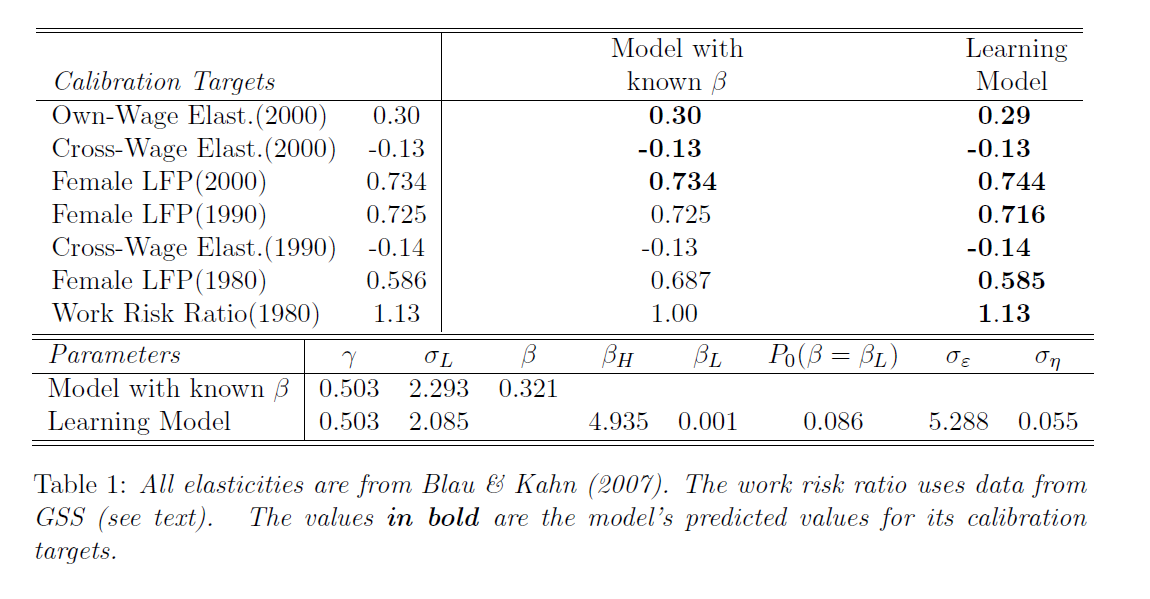
\includegraphics[width=0.8\textwidth]{Table1.png}
    \label{fig:Table 1}
  \end{table}

 All elasticities are from Blau and  Kahn (2007). The work risk ratio uses data from GSS (see text). The values in bold are the model's predicted values for its calibration
targets. 
  
\begin{figure}[H]
  \centering
  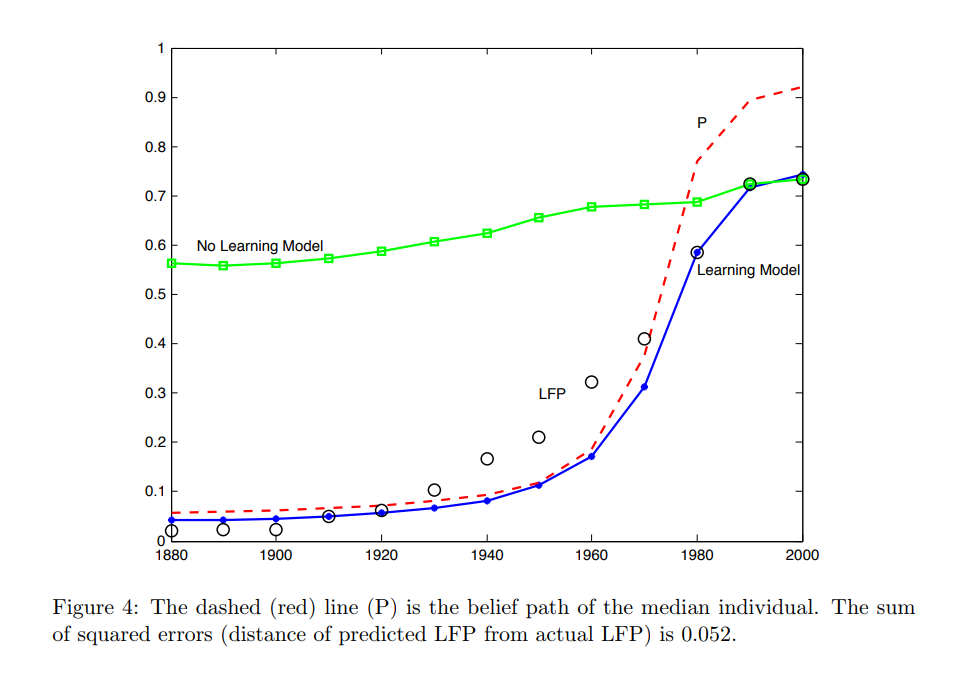
\includegraphics[width=1\textwidth, height=10cm]{Figure4.png}
  \caption{}
    \label{fig:Figure 4}
  \end{figure}

The dashed (red) line (P) is the belief path of the median individual. The sum of squared errors (distance of predicted LFP from actual LFP) is 0.052. 

\hypertarget{Simulation Results}{}
\section{Discussion and Conclusion}

 In the model, married women compared the benefits of increased consumption from labor earnings with the expected utility cost of working.

This cost was unknown and women's beliefs about it evolved endogenously over time in a Bayesian fashion.

The calibrated model finds that at the outset women were pessimistic about the true cost of working.

The paper shows that a simple model with these features, calibrated to key statistics from the later part of the 20th century, generates a time trend of married women's LFP that is roughly similar to the historical one in the US over the last 120 years.


\clearpage\vfill\eject

\onlyinsubfile{\bibliography{\econtexRoot/LaTeX/BufferStockTheory,economics}}

\end{document}

